\documentclass{workbook}

%\solutionfalse
\solutiontrue

\coverimage{images/escher.jpg}
\departmentlogo{example-image-a}
\coursenumber{Subject 1234}
\coursename{Course title}
\coursesemester{Summer 2077}
\instructorname{Firstname Lastname}

\addbibresource{references.bib}

\epigraph{
    There is a theory which states that if ever anyone discovers exactly what the Universe is for and why it is here, it will instantly disappear and be replaced by something even more bizarre and inexplicable.
    
    There is another theory which states that this has already happened.
    
}




\begin{document}
	
	\maketitle
	
	\frontmatter
	
	\makeepigraph

	\tableofcontents
	
%%%%%%%%%%%%%%%%%%%%%%%%%%%%%%%%	
    
    \chapter*{Acknowledgement}

%%%%%%%%%%%%%%%%%%%%%%%%%%%%%%%%	
	
	\FrontMatter{Introduction}\label{chapter:introduction}

The History of every major Galactic Civilization tends to pass through three distinct and recognizable phases, those of Survival, Inquiry and Sophistication, otherwise known as the How, Why, and Where phases. For instance, the first phase is characterized by the question `How can we eat?' the second by the question `Why do we eat?' and the third by the question `Where shall we have lunch?

%%%%%%%%%%%%%%%%%%%%%%%%%%%%%%%%	

	\mainmatter
	
%%%%%%%%%%%%%%%%%%%%%%%%%%%%%%%%	
	
	\chapter{How to use this template}

\section{First Section}

Uses kpfonts.

\begin{defn}[Definition Title]{label_defn1}
	A definition. The title is optional.
\end{defn}



\begin{exmpl}[Title]{label_exmpl}
	\begin{itemize}
		\item First example 
		\begin{itemize}
			\item  Note $1$
			\item  Note $2$
		\end{itemize}
		\item Second example
	\end{itemize}
\end{exmpl}    



Some other text.

\begin{theo}[Theorem Title]{label_thm}
	A Theorem that uses objects defined in \cref{label_defn1}. Title is optional. 
	\[\dint_a^b u v' \dx = [u(x)v(x)] \eval_a^b - \dint_a^b u'(x) v(x) \dx\]
\end{theo}


\begin{prf}{label_thm}
	Proof text ends in qed symbol. Must be supplied the label of the theorem.
\end{prf}


\begin{exercise}[Questions have their own counters.]\label{question_label}
	\begin{enumerate}
		\item Greek letters and uppercase math letters are always upright. Such as \label{step_a}
		\begin{enumerate}
			\item  $\alpha x^2 +\beta$ \label{substep_a_i} 
			\item  $y =mx+ C \in \R$ 
		\end{enumerate}
		
		\item Do the  following tasks after \ref{step_a}.
		\begin{tasks}(3)
			\task first do \ref{substep_a_i}.
			\task ??    
			\task Profit
		\end{tasks}
\end{enumerate}
\end{exercise}

\begin{solution}
	Solution to the exercise. Uncomment the ``solutionfalse'' flag to make solutions invisible.
\end{solution}


\begin{note}[Fun Fact:]
	This is a note with a custom title. Default is `Note:'.
\end{note}



\section{Second Section}

Let's start with a picture that explains the main idea:
\begin{figure}[!ht]
    \centering
    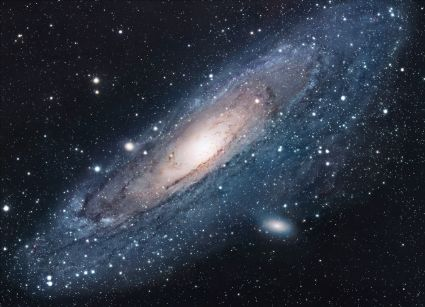
\includegraphics[width=0.5\textwidth]{images/universe.jpg}
    \caption{The Universe}
    \label{fig:universe}
\end{figure}


\begin{axiom}{label_axiom}
	This is an axiom.
\end{axiom}

\begin{prop}{label_proposition}
	This is a proposition.
\end{prop}

\begin{claim}{label_claim}
	This is a claim.
\end{claim}

\begin{digression}
	A digression into tangentially related topics.
\end{digression}



\subsection{Case 1: First subsection}
When  \cref{label_exmpl} is true.
\begin{warning}[A Warning:] %default is Warning:
	\lipsum[1][1-2]
\end{warning}

\subsection{Case 2: Second subsection}
Do \cref{question_label} first.

Computer Code is written as {\tt Typewriter font}.

\begin{code}{Python}
    def rk4(f,x0,t0,tmax,dt):
        t = # build the time array
        x = # initialize an empty array for the x values
        x[0] = # build the initial condition
        # On the next line: be careful about how far you're looping
        for i in range( ??? ):
        # The interesting part of the code goes here.
        # Start from t[i] and x[i]. Then Define k1, k2, k3, k4 
        # and use them to find x[i+1]
        return t, x
        
    f = lambda t, x: # the definition of the function goes here
    
    x0 = # initial condition
    t0 = 0
    tmax = # your choice
    dt = # pick something reasonable
    t, x = rk4( ??? , ??? , ??? , ??? , ??? )
    # plot t vs. x
\end{code}

	
	\chapter{How to write in \LaTeX}

\section{Important Stuff}

This section contains some important information about writing in \LaTeX.

\subsection{Notes about Quotes and Internal references}

When you quote something in \LaTeX, you have to do it like ``this.''
If you do it like ''this,'' one of your quotation marks will be backwards.

Another nice thing about using \LaTeX \ is that you can reference 
equations and figures once you have labeled them. For example,
\cref{fig:universe} is a picture of the universe! You can also 
reference equations, sections, lemmas, theorems, etc. See the
examples in \cref{sec:moremath}.



\subsection{More Math Stuff}
\label{sec:moremath}

Mathematical expressions, like $x^{2} + 3$, are easy to create in \LaTeX.
It is also easy to have a formula written on a separate line, like \[x^{2} + 3 = 0.\]



Numbered equations are easy too!
\begin{equation}
	\label{eq:simpleequation}
	x^{5} - 9x^{4} = \sin 3.
\end{equation}
You can also refer to previous equations.
The formula
\begin{equation}
	x = \frac{-b \pm \sqrt{b^{2} - 4ac}}{2a} \label{yourlabel}
\end{equation}
is the quadratic formula.
You can use \cref{yourlabel} to solve quadratic equations.

% Notice that you can also place equations and formulas between the commands 
% ''\begin{equation}'' and ''\end{equation}''. No dollar signs are necessary in this case. 

% You can also create a label for the equation using the command ''\label''. You can 
% refer back to the equation using the ''\ref'' command. Notice how LaTeX 
% automatically takes care of the numbering. When you use the ''\ref'' command, you 
% will need to run LaTeX on the source file twice. This is necessary so that LaTeX 
% can keep track of the numbering. (Note that LaTeX will complain a little bit the first 
% time you run the source file through. This is not serious.)

Here is a formula with some simple mathematical operations:
\[5 \times 3 + 4 \div 2 = 2 \cdot 10 - 3 < 100.\]
Another simple formula:
\[x^{2} \geq 0.\]		% The command ''\geq'' is ''greater than or equal'' and 
% ''\leq'' is ''less than or equal''.				
This formula is true for $x \in \mathbb{R}$.	% The command ''\mathbb'' specifies 
% a certain type of math font. There are 
% also the ''\mathbf'' (bold) and the 
% ''\mathcal'' (calligraphic) commands, 
% among others, for specifying font styles 
% in math formulas.
One more simple formula:
\[0 \neq \frac{\pi}{2}.\]
Some simple trigonometry:
\[\sin(2x) = 2 \sin x \cos x.\]
Some simple logarithms:
\[\log(x) = \frac{\ln x}{\ln 10}.\]


And now some Greek letters:
\[\alpha + \beta = \gamma.\]
A formula involving set notation:
\[A \cup (B \cap C) = (A \cup B) \cap (A \cup C).\]
The derivative:
\[\lim_{h \rightarrow 0}\frac{f(x + h) - f(x)}{h} = f'(x).\]
The Riemann sum
\[\sum_{i = 1}^{n}f(x_{i})\Delta x\]
approximates the integral
\[\int_{a}^{b}f(x)\;dx.\]		% The characters ``\;'' just place some additional space 
% in the formula.
Finally, an infinite series:
\[1, \frac{1}{2}, \frac{1}{4}, \ldots.\] %Also try \cdots





\section{Conclusion}
``I always thought something was fundamentally wrong with the universe.'' \cite{adams1995hitchhiker}



	\backmatter
	
%%%%%%%%%%%%%%%%%%%%%%%%%%%%%%%%	

	\appendix
	\addcontentsline{toc}{chapter}{Appendices}
	\chapter*{Appendices}
	\renewcommand{\thesection}{\Alph{section}}
	
	
%%%%%%%%%%%%%%%%%%%%%%%%%%%%%%%%
    \section{First Appendix}
	
%%%%%%%%%%%%%%%%%%%%%%%%%%%%%%%%
%%%%%%%%%%%%%%%%%%%%%%%%%%%%%%%%

    \addcontentsline{toc}{chapter}{Exercises}
	\chapter*{Exercises}
    
%%%%%%%%%%%%%%%%%%%%%%%%%%%%%%%%

	\setcounter{question}{1000}
	\section{Weekly Exercises}

\solutionfalse
% \solutiontrue

\begin{exercise}
    This is an exercise.
\end{exercise}


   
%%%%%%%%%%%%%%%%%%%%%%%%%%%%%%%%%%%%%%%%


    
    \nocite{*}
	\printbibliography[title={Resources},heading=bibintoc]
	
\end{document}	

